\scanpage{135}

Théorème de \handwritten{- - - - - -} (rapporté par Husemöller).

Soit $A$ une bialgèbre sur le corps $k$, $A$ associative et unitaire pour ses deux structures, ``cocomplète'' pour sa filtration canonique de comodule (duale de la filtration par les puissances de l'idéal d'augmentation du dual; de façon précise, écrivant $\overset{n}{\otimes}A=\overset{n}{\otimes}A^{\handwritten{+}}+$ fou\uline{r}bis, d'où via la m.ème itéré\deleted{\unsure{e|s}} du morphisme diagonal, une application $A\handwritten{\longrightarrow}\overset{n}{\otimes}I^{\handwritten{+}}$, dont le noyau\inserted{\handwritten{\unsure{intersect°|intersect.} avec $A^{+}$}} est $\mathrm{Filt}_{m}(A)$).\margin{\handwritten{cela entraîne qu'il y a un \unsure{antipodisme} ?}} (NB l'hypothèse cocomplète est satisfaite pour une coalgèbre \inserted{avec unité} à degrés $\handwritten{\geq}$ $0$ réduite à $k$ en degré\deleted{s} $0$, associative et unitaire, - parait-il !). Soit $M$ un $A$-module, muni d'un homomorphisme diagonal \inserted{sur $k$} unitaire (peut-être pas associatif), $M\handwritten{\longrightarrow}M\otimes_{k}M$, qui soit $A$-linéaire\unsure{,|.}\margin{\figure{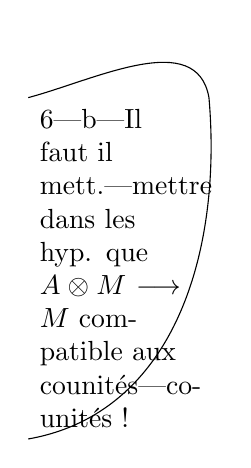
\begin{tikzpicture}
\node[text width=2cm,inner sep=4pt] (n) {\handwritten{\unsure{6|b|Il} faut il \unsure{mett.|mettre} dans les hyp. que $A\otimes M\longrightarrow M$ compatible aux \unsure{counités|co-unités} !}};
\draw (n.north west) to[out=15,in=100] (n.north east) to[out=-85,in=10] (n.south west);
\end{tikzpicture}}}\inserted{\handwritten{(pour la structure de $A$-module sur $M\otimes M$ provenant de $A\longrightarrow A\otimes A$; il revient au même de dire que $A\otimes M\longrightarrow M$ comp. avec application diagonale)}} Supposons de plus donné une ``unité'' i.e. un homomorphisme $k\handwritten{\longrightarrow}M$ qui soit un homomorphisme de coalgèbres unitaires, i.e. $\underset{M}{\mathrm{L}}$'image $\inserted{e_{M}}$ de $1$ satisfait $\handwritten{\unsure{\epsilon|\varepsilon}}_{M}(e_{M})=1$, $\handwritten{\Delta}_{M}(e_{M})=e_{M}\otimes e_{M}$. Supposons également $M$ cocomplète, et que\deleted{on} l'application $u\handwritten{\mapsto}u.e$ de $A$ dans $M$ soit injective. Alors $M$ est un $A$-module libre, \inserted{\handwritten{ayant une base dont fait partie $e$;}} de façon plus précise, posant $\overset{\handwritten{-}}{M}=M\otimes_{A}k$, il existe un isomorphisme (non canonique ...) de $A$-modules $M\handwritten{\overset{\sim}{\unsure{\longleftarrow|\longleftrightarrow}}}A\otimes_{k}\overset{\handwritten{-}}{M}$\handwritten{, tel que le diagramme}
\margin{\handwritten{?}}
\handwritten{\diagram{\begin{tikzcd}[ampersand replacement=\&,column sep=small,row sep=small]
M \arrow[dr] \& \& \unsure{A|\mathcal{A}}\otimes_{k}\overline{M} \arrow[ll,"\sim"'] \arrow[dl] \\
\& \overline{M} \&
\end{tikzcd}}}
\handwritten{\unsure{commute|commuta}, et que ...}

Exemple \handwritten{1}. Supposons l'application diagonale de $A$ commutative. Alors $A$ peut être considéré comme l'hyperalgèbre d'un groupe formel connexe $\inserted{G}$ sur $k$. Si $\handwritten{\Delta}_{M}$ est associatif et commutatif, $M$ aussi est formé des distributions à l'origine d'une variété formelle connexe $\inserted{V}$ sur $k$, et le fait que $A$ opère sur $M$ de façon que l'application diagonale soit $A$-linéaire signifie que $G$ opère sur $V$. On voit donc que si $u\handwritten{\unsure{\vdash|\mapsto}}\unsure{\mathbb{U}|\mathbb{u}|U|u}.e$ \inserted{de $A$ dans $M$} est injectif, i.e. si $g\handwritten{\mapsto}g.a$ ($a$ le `centre' de $V$) de $G$ dans $V$ est un monomorphisme, alors $M$ est libre sur $A$. En fait, on trouvera que $G$ opère librement sur $V$ i.e.
% archive sheet number: 134
